
%% CLASS MANUAL FOUND IN http://blog.poormansmath.net/latex-class-for-lecture-notes/ %%
%% CLASS AUTHOR Stefano Maggiolo %%

%%%%%%%%%%%%%%%  TITLE PAGE  %%%%%%%%%%%%%%%%%%%
\documentclass[english,course]{Notes}
\title{COURSE CODE}
\subject{SUBJECT AREA}
\author{Joao Almeida-Domingues}
\email{2334590D@student.gla.ac.uk}
\speaker{LECTURER}
\date{13}{01}{2020}
\dateend{25}{03}{2020}
\place{University of Glasgow}


%%%%%%%%%%%% BIB CONFIG %%%%%%%%%%%%%%%
\usepackage[backend=biber, style=reading]{biblatex} 

\bibliography{OOSE} %add bib file name

%%%%%%%%%%% LAYOUT  %%%%%%%%%%%%%%%

\renewcommand{\abstractname}{\vspace{3\baselineskip}} %hack to remove abstract


%%%%%%%%%%%%%%%%%%%%%%%%%%%%%%%%

%%%%%%%%%%%%%% KEEP HERE (conflict when in class) %%%%%%%%%%%%%%%%%%%%

 %%%%%MATRICES
    
    \let\mat=\spalignmat
    \let\amat=\spalignaugmat
    \let\vec=\spalignvector
    
%%%%%% row ops
    \newcommand\ro[2]{\xrightarrow[#2]{#1}}
%%%%%%%%%%%%%%%%%%%%%%%%%%%%%%%%%%%%%%%%%%%%%%%%%%%%%

%%%%%%%%%%%%%  PACKAGES (NOT INCLUDED IN CLASS) %%%%%%%%%%%%%%
\usepackage[delims={[]}]{spalign}

%%%%%%%%%%%%%%%% ALGORITHM TEMPLATE %%%%%%%%%%%%%%%%%%%%

%\begin{algorithm}[H]
%\SetAlgoLined\KwData{this text}
%\KwResult{how to write algorithm with \LaTeX2e }initialization\;
%\While{not at end of this document}
%	{read current\;\eIf{understand}{go to next section\;current section becomes this one\;}{go back to the beginning of current section\;}}
%	\caption{How to write algorithms}
%\end{algorithm}

%%%%%%%%%%%%%%%%%%%%%%%%%%%%%%%%%%%%%%%%%%%%%%%%%%%%%

\begin{document}

%%%%%%%%%%%%%%  DISCLAIMER  %%%%%%%%%%%%%%%%%%%%%

\begin{abstract}
	\par{These lecture notes were collated by me from a mixture of sources , the two main sources being the lecture notes provided by the lecturer and the 
content presented in-lecture. All other referenced material (if used) can be found in the \ita{Bibliography} and \ita{References} sections.}
	\par{The primary goal of these notes is to function as a succinct but comprehensive revision aid, hence if you came by them via a search engine , please note 
that they're not intended to be a reflection of the quality of the materials referenced or the content lectured.}
	\par{Lastly, with regards to formatting, the pdf doc was typeset in \LaTeX , using a modified version of Stefano Maggiolo's \href{http://blog.poormansmath.net/
latex-class-for-lecture-notes/}{\underline{\textcolor{blue}{class}}}}
\end{abstract}
\newpage

%%%%%%%%%%%%% LECTURES %%%%%%%%%%%%%%%%%%%%%%%


\section{Modelling}

\lecture{13}{01}{20}
	\key{Object}{Encapsulation}{Polymorphism}{Inheritance}{Abstraction}{Class}{Methods}{Attributes}{End-User}

	\par{This course will focus on the basic concepts of OOP. The main idea
being that one can model real world objects as abstractions in software. We take
the object's attributes and functions and convert them into a single entity
consisting of data and methods which operate on that data}

\subsection{3 Principles of OOP}

	\defn{Encapsulation}{when data and operations exist within the same entity}
	\defn{Inheritance}{classes can inherit attributes and methods from other
classes}
	\defn{Polymorphism}{ability of an entity to take many forms}

	\par{As seen in JP2, the data and methods are defined within the class, and
are often protected from outside access unless via getter and setters. If a
class is a subset of another class then it inherits all (or most) of its
behaviours and attributes and so it can be \ita{subclassed}. This ability of the
superclass to take many forms depending on which child is called is one of the
crucial aspects of OOP. When methods are \ita{overridden} by child class a
method of an object reference to a superclass is invoked at compile time, and it
is later dispatched to the overridden of the specific class instance at run time} 

\subsection{OO Design}

	\par{Software design relies on a symbiotic relation between the end-user and
the designer. Often one is given a spec/problem statement by a client, or given
a certain user story (recall HCI:1F) and from there the designer will use its
modelling knowledge to interpret it in the light of OOP paradigms}
	
\begin{enumerate}
	\item Identify real world objects (look at the nouns in the spec)
	\item Identify relationships between objects
		\begin{enumerate}
			\item[] Generalization : Abstract common features (e.g \ita{move})
			\item[] Containment : Object A $\subseteq$ B (e.g \ita{Dog} $\subset$
					\ita{Animal})
			\item[] Multiplicity : Quantity relation (e.g Dog (1)
					$\leftrightarrow$ (Many) Paws)
		\end{enumerate}
	\item{Identify operations and associate them with objects (this is usually
		done by looking at the verbs in the spec)}
	\item{Create an Interface}
		\begin{itemize}
			\item[]{it is essentially a contract which guaranteed that each object
					represented by a given class will behave in a specified manner}
			\item[]{it must include a \ita{return type} ,
\ita{purpose/description} , \ita{pre-conditions} , i.e what must be true prior
to the method being called , \ita{post-conditions} , what must be true when
returning}
		\end{itemize}
		\item{Object Encapsulation , which describes how objects communicate
		via operations and how this affects the end-user} 
\end{enumerate}

\subsection{UML}

	\defn{Design}{specify the structure of a system and its behaviour}

	\defn{Domain Model}{conceptual model of the domain that includes both data
	and behaviour}

	\par{When designing software we go from \ita{"what"} to \ita{"how"}, i.e. we
			worry about how we can represent real world systems in software. In
	particular, how we can use classes, fields etc. Out of this process a
	\ita{domain model} emerges which represents, at the required level of
	formality, the system with concepts, roles and their interaction}

	\par{\ita{UML} is an open standard language created to represent
			diagrammatically an OO system. It has a \ita{descriptive} side which
			provides a formal syntax as well as a more flexible
	\ita{prescriptive} one, where usage shapes conventions}
	\par{Given this flexibility UML has several uses, from providing a sketch of
		 the software, which can be used to give the client an idea of the
		 current stage of the design, and improve upon it given her feedback
		 (e.g \ita{use cases} modeling) or more like a blueprint, where the complete
 design is given to engineers for implementation.}
	
 \subsubsection{Class Diagrams}

	\defn{Class Diagrams}{represent the classes in an OO system, their fields,
	methods and their interactions}
	\par{\mymarginpar{Pros \& Cons} In this course we'll focus on class diagrams, which focus on the
	representation of classes. These are particularly good for providing an
	overview of the data and attributes, as well as the main entities in play in
	the design along with the complexity of their interaction. They are however
	not adequate for prying into the logic of the program or its control flow.}
	
	\par{Given the wide adoption of the language in industry, the following
	conventions were adopted:}

	\begin{enumerate}
		\item Name
				\begin{itemize}
						\item Name : top of the box
						\item Interfaces : in between \texttt{<< >>}
						\item Abstract : italics
				\end{itemize}
		\item Methods
				\begin{itemize}
						\item Methods : \texttt{mName(arg:type)}
						\item Getter/Setter : may be ommited
						\item Interface : do not omit
						\item Inherited : omit
						\item Return : omit if constructor or void
				\end{itemize}
		\item Attributes
				\begin{itemize}
						\item Signature : \texttt{visibility name : type}
						\item Derived : \texttt{/}~\mymarginpar{not stored, but
								can be computed from other attributes (e.g area,
						given width and height attributes)}
				\end{itemize}
		\item Visibility
				\begin{itemize}
						\item Public/Private : \texttt{+ / -} 
						\item Protected/Package : \texttt{\# / $\sim$}
						\item Static : underlined
				\end{itemize}	
		\item Generalization Relationships
				\begin{itemize}
						\item Top-Down i.e , Parent-Child
						\item Class : Solid line , black head
						\item Abstract : Solid line, white head
						\item Interface : dashed
				\end{itemize}
		\item Usage Relationships
				\begin{itemize}
						\item Multiplicity : * = 0+ , m..n = [m,n]
						\item Navigability : Yes \texttt{->} , No X
						\item Aggregation : White diamond
						\item Composition : Black Diamond
						\item Dependency : Dotted 
				\end{itemize}
	\end{enumerate}

	\defn{Generalization Relationships}{represent inheritance and interfaces}

	\defn{Association Relationships}{used to show that instances of classifiers
			could be either linked to each other or combined logically or
	physically into some aggregation}

	\par{There are 3 major types of associational/usage relationships classified
			by the degrees to which the related entities are linked. So,
			dependent types represent a \ita{"uses temporarily"} relation ;
			aggregation represent \ita{"is part of"} and composition
	represents an \ita{"is entirely made of"}.}
	\par{To illustrate the differences between them take the "engine-car"
			relation. We say that the engine is part of the car, and the car has
			an engine. A stronger relation would be that of a book and its
			pages. Note that it is conceivable to image a car without a motor, a
			car would still be a car, even if it lost its motor. However, what
			is a book without pages? Lastly, the dependency relation are the
			weakest connectors, and simply state a sort of relation where
	one object \ita{might} use another. It is often an implementation detail,
	not an intrinsic part of the object itself (e.g. \ita{hasRead} method in
	\ita{Person} and a \ita{Book} object)}

	\begin{figure}[H]
			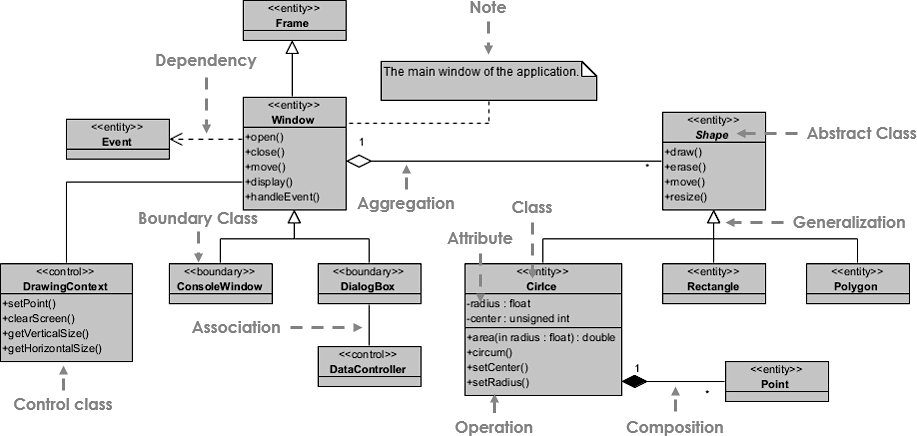
\includegraphics[width=\textwidth]{uml.png}
			\caption{GUI Class Diagram \cite{umlVisual}}
	\end{figure}





%%%%%%%%%%%%%%  BIBLIOGRAPHY  %%%%%%%%%%%%%%%%%%%
\newpage
\nocite{*}
\printbibliography

%%%%%%%%%%%%%%%%%%%%%%%%%%%%%%%%%%%%%%%%%%

\end{document}
